\documentclass[a4paper,12pt]{article}
\usepackage[indonesian]{babel}
\usepackage{graphicx}
\usepackage{multirow}
\usepackage{enumitem}
\usepackage{listings}
\usepackage{wrapfig}
\usepackage[T1]{fontenc}
\usepackage{inconsolata}
\usepackage{lipsum}
\usepackage{adjustbox}


\usepackage{color}
\usepackage[table]{xcolor}
\definecolor{mygreen}{rgb}{0,0.6,0}
\definecolor{mygray}{rgb}{0.5,0.5,0.5}
\definecolor{mymauve}{rgb}{0.58,0,0.82}
\lstset{%
    language=java,
    showstringspaces=false,          % Prevent tex replacing space to bracket in code
    frame=single,                    % Set frame around code
    backgroundcolor=\color{white},   % choose the background color
    basicstyle=\footnotesize,        % size of fonts used for the code
    breaklines=true,                 % automatic line breaking only at whitespace
    captionpos=b,                    % sets the caption-position to bottom
    commentstyle=\color{mygreen},    % comment style
    keywordstyle=\color{blue},       % keyword style
    stringstyle=\color{mymauve},     % string literal style
}

\graphicspath{ {./img/} }
\begin{document}
\title{ {\Large Laporan Praktikum}\\ Algoritma dan Pemrograman Lanjut\\{\Large Pertemuan 5}}

\author{Aldzikri Dwijayanto Prathama
    \\195410189
    \\Informatika}
\makeatletter
\begin{titlepage}
    \begin{center}
        {\huge \bfseries \@title}\\[14ex]
        
\includegraphics[scale=.8]{logo}\\[4ex]
        {\large \@author}\\[12ex]
        {\large \bfseries {SEKOLAH TINGGI MANAJEMEN INFORMATIKA DAN KOMPUTER
            AKAKOM YOGYAKARTA}}
    \end{center}


%{\large \@date}
\end{titlepage}
\makeatother
%\maketitle
\newpage
\tableofcontents
\newpage

\section{Tujuan}
\paragraph{}
Mahasiswa dapat:
\begin{enumerate}
    \item Menjelaskan konsep array 3 dimensi
    \item Merencanakan struktur data dalam bentuk array 3 dimensi
    \item Mengaplikasikan array 3 dimensi
\end{enumerate}


\section{Teori}
\paragraph{}
Array 3 dimensi adalah array yang tidak jauh berbeda dari array
dimensi satu dan dua yang telah dijelaskan sebelumnya, kecuali pada indeks
dari array. Pada tipe ruang misalnya type ruang = array [1..8,1..5,1..3] of
integer; menunjukkan bahwa ruang adalah nama-pengenal/variabel yang
berupa array yang komponennya bertipe integer dan terdiri atas 8 baris,
mempunyai 5 kolom dan 3 halaman.

\newpage

\section{Pembahasan}
\subsection{Praktik}
\subsubsection{Praktik 1}
\begin{lstlisting}
import java.util.Scanner;

public class NilaiUjianSiswa {
    public static void main(String[] args) {
        double[][][] nilai = {
                { { 51.58, 89.94 }, { 60.06, 59.58 }, { 52.93, 47.63 }, { 89.98, 77.56 }, { 45.87, 94.56 } },
                { { 39.46, 58.41 }, { 71.42, 85.37 }, { 39.08, 78.21 }, { 79.03, 80.32 }, { 45.49, 23.47 } },
                { { 81.09, 32.24 }, { 51.86, 86.92 }, { 59.58, 31.69 }, { 96.18, 26.72 }, { 28.76, 91.54 } } };
        for (int i = 0; i < nilai.length; i++) {
            for (int j = 0; j < nilai[0].length; j++) {
                for (int k = 0; k < nilai[0][0].length; k++) {
                    System.out.print("nilai[" + i + "][" + j + "][" + k + "] = " + nilai[i][j][k] + "\t");
                }
                System.out.println();
            }
            System.out.println();
        }
    }
}
\end{lstlisting}
Praktik 1 adalah memiliki array 3 dimensi yang datanya berbentuk double, yang memiliki 1 halaman, 5 baris, dan 2 kolom. Setelah itu terdapat perulangan for
yang akan mengeprint isi dari variabel nilai.
\begin{center}
    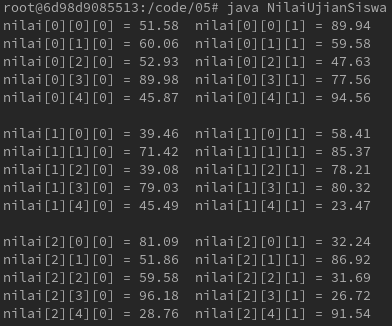
\includegraphics[scale=.8]{1.png}
\end{center}

\subsubsection{Praktik 2}
\begin{lstlisting}
import java.util.Scanner;

public class NilaiUjianSiswa1 {
    public static void main(String[] args) {
        double[][][] nilai = {
                { { 51.58, 89.94 }, { 60.06, 59.58 }, { 52.93, 47.63 }, { 89.98, 77.56 }, { 45.87, 94.56 } },
                { { 39.46, 58.41 }, { 71.42, 85.37 }, { 39.08, 78.21 }, { 79.03, 80.32 }, { 45.49, 23.47 } },
                { { 81.09, 32.24 }, { 51.86, 86.92 }, { 59.58, 31.69 }, { 96.18, 26.72 }, { 28.76, 91.54 } } };
        System.out.println("Array nilai ditampilkan: ");
        for (int i = 0; i < nilai.length; i++) {
            for (int j = 0; j < nilai[0].length; j++) {
                for (int k = 0; k < nilai[0][0].length; k++) {
                    System.out.print("nilai[" + i + "][" + j + "][" + k + "] = " + nilai[i][j][k] + "\t");
                }
                System.out.println();
            }
            System.out.println();
        }
        // Menghitung nilai rata-rata
        System.out.println("Nilai rata-rata siswa: ");
        for (int i = 0; i < nilai.length; i++) {
            double totalNilaiPilihanGanda = 0, totalNilaiEssay = 0;
            for (int j = 0; j < nilai[0].length; j++) {
                totalNilaiPilihanGanda += nilai[i][j][0];
                totalNilaiEssay += nilai[i][j][1];
            } // Menampilkan hasil
            double pilihanGanda = totalNilaiPilihanGanda / nilai[0].length;
            double essay = totalNilaiEssay / nilai[0].length;
            System.out.printf("Nilai rata-rata ujian soal pilihan ganda siswa " + (i + 1) + " adalah %4.2f \n", pilihanGanda);
            System.out.printf("Nilai rata-rata ujian soal essay siswa " + (i + 1) + " adalah %4.2f \n", essay);
            System.out.println();
        }
    }
}
\end{lstlisting}
Program tersebut merupakan program dari praktik 1 yang dimodifikasi dengan menambahkan perulangan yang akan menjumlahkan nilai siswa, kemudian akan membaginya
dengan panjang data dari variabel untuk mencari rata-rata dari niali siswa.
\begin{center}
    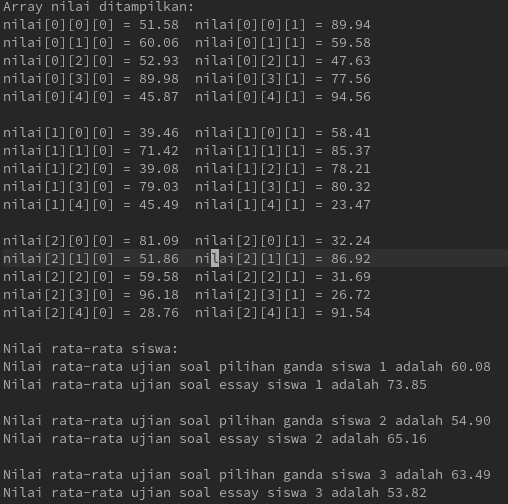
\includegraphics[scale=.8]{2.png}
\end{center}

\subsubsection{Praktik 3}
\begin{lstlisting}
import java.util.Scanner;

public class InisialisasiArray3D {
    public static void main(String args[]) {
        Scanner input = new Scanner(System.in);
        System.out.println("Masukkan jumlah siswa: ");
        final int JUMLAH_SISWA = input.nextInt();
        System.out.println("Berapa kali ujian dilakukan: ");
        final int JUMLAH_UJIAN = input.nextInt();
        double[][][] nilai = new double[JUMLAH_SISWA][JUMLAH_UJIAN][2];
        System.out.println("Silakan masukkan data: ");
        // Membaca nilai yang diinput oleh user
        for (int a = 0; a < JUMLAH_SISWA * JUMLAH_UJIAN; a++) {
            int nomorSiswa = input.nextInt();
            int nomorUjian = input.nextInt();
            double nilaiPilihanGanda = input.nextDouble();
            double nilaiEssay = input.nextDouble();
            nilai[nomorSiswa - 1][nomorUjian - 1][0] = nilaiPilihanGanda;
            nilai[nomorSiswa - 1][nomorUjian - 1][1] = nilaiEssay;
        }
        // Menampilkan array
        System.out.println("Array nilai ditampilkan: ");
        for (int i = 0; i < nilai.length; i++) {
            for (int j = 0; j < nilai[0].length; j++) {
                for (int k = 0; k < nilai[0][0].length; k++) {
                    System.out.print("nilai[" + i + "][" + j + "][" + k + "] = " + nilai[i][j][k] + "/t");
                }
                System.out.println();
            }
            System.out.println();
        }
        // Menghitung nilai rata-rata
        System.out.println("Nilai rata-rata siswa: ");
        for (int i = 0; i < nilai.length; i++) {
            double totalNilaiPilihanGanda = 0, totalNilaiEssay = 0;
            for (int j = 0; j < nilai[0].length; j++) {
                totalNilaiPilihanGanda += nilai[i][j][0];
                totalNilaiEssay += nilai[i][j][1];
            }
            // Menampilkan hasil
            double pilihanGanda = totalNilaiPilihanGanda / nilai[0].length;
            double essay = totalNilaiEssay / nilai[0].length;
            System.out.printf("Nilai rata-rata ujian soal pilihan ganda siswa " + (i + 1) + " adalah %4.2f /n", pilihanGanda);
            System.out.printf("Nilai rata-rata ujian soal essay siswa " + (i + 1) + " adalah %4.2f /n", essay);
            System.out.println();
        }
    }
}
\end{lstlisting}
Untuk praktik 3 adalah memodifikasi dari praktik 2 yang dimodifikasi sehingga program bisa menerima inputan dari user. Untuk memasukkan nilai ke dalam variabel
array digunakan perulangan for.
\begin{center}
    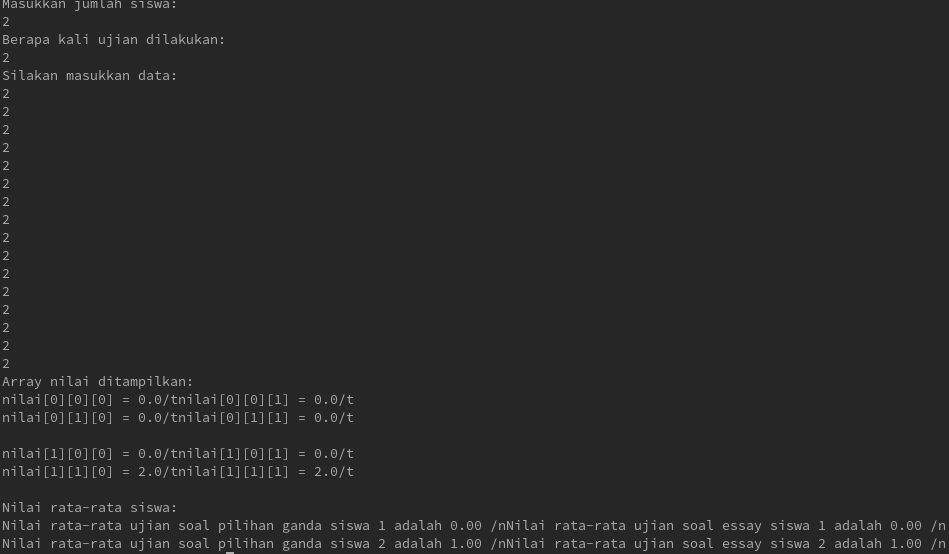
\includegraphics[width=\linewidth]{3.png}
\end{center}

\subsection{Latihan}
\subsubsection{Latihan 1}
\begin{lstlisting}
public class ArrayMultidimensi {
    public static void main(String[] args) {
        String entry[][][] = { { { "vianslezer", "100411052", "Surabaya" }, { "Echa", "100411025", "Jakarta" },
                { "Masayu", "100411024", "Malang" } } };
        System.out.println("Nama : " + entry[0][0][0]);
        System.out.println("Nim : " + entry[0][0][1]);
        System.out.println("Alamat : " + entry[0][0][2]);
        System.out.println("-------------------------");
        System.out.println("Nama : " + entry[0][1][0]);
        System.out.println("Nim : " + entry[0][1][1]);
        System.out.println("Alamat : " + entry[0][1][2]);
        System.out.println("-------------------------");
        System.out.println("Nama : " + entry[0][2][0]);
        System.out.println("Nim : " + entry[0][2][1]);
        System.out.println("Alamat : " + entry[0][2][2]);
        System.out.println("-------------------------");
    }
}
\end{lstlisting}
Program untuk latihan tersebut memiliki array yang tiga dimensi yang memiliki 1 halaman, 3 baris, dan 3 kolom. Kemudian program akan menampilkan isi dari array
tersebut tanpa menggunakan perulangan.
\begin{center}
    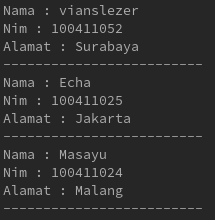
\includegraphics[scale=.8]{4.png}
\end{center}

\subsubsection{Latihan 2}
\begin{lstlisting}
import java.util.Scanner;

public class Latihan2 {
    public static void main(String[] args) {
        Scanner input = new Scanner(System.in);
        System.out.print("Masukkan banyak data = ");
        int batas = input.nextInt();
        String[][][] entry = new String[1][batas][3];
        for (int i = 0; i < batas; i++) {
            for (int j = 0; j < 3; j++) {
                if (j == 0) {
                    input.nextLine();
                    System.out.print("Nama = ");
                    entry[0][i][j] = input.nextLine();
                } else if (j == 1) {
                    System.out.print("Nim = ");
                    entry[0][i][j] = input.nextLine();
                } else {
                    System.out.print("Alamat = ");
                    entry[0][i][j] = input.nextLine();
                }
            }
        }
        input.close();
        System.out.println();
        for (int i = 0; i < batas; i++) {
            for (int j = 0; j < 3; j++) {
                if (j == 0) {
                    System.out.println("Nama    \t: " + entry[0][i][j]);
                } else if (j == 1) {
                    System.out.println("Nim    \t: " + entry[0][i][j]);
                }
                else {
                    System.out.println("Alamat    \t: " + entry[0][i][j]);
                }
            }
            System.out.println("-----------------------------------");
        }
    }
}
\end{lstlisting}
Untuk latihan kedua, adalah memodifikasi latihan 1 agar program bisa dimasukkan lebih dari 5 data. Untuk memasukkan data ke dalam variabel array tersebut
digunakan perulangan for. Didalam perulangan terdapat pernyataan seleksi di dalam perulangan tersebut, yang berguna untuk menginstruksikan user, untuk
memasukkan nama, NIM, atau alamat. Setelah user selesai memasukkan data program akan menampilkan data yang sudah dimasukkan dengan perulangan for.
\begin{center}
    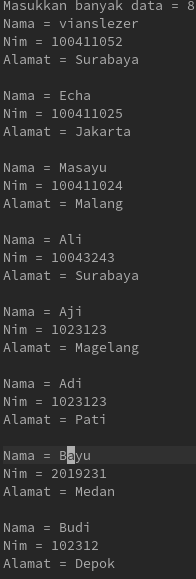
\includegraphics[scale=.45]{5.png}
    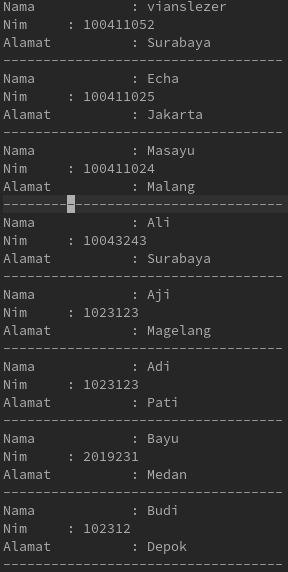
\includegraphics[scale=.45]{5a.png}
\end{center}

\subsubsection{Latihan 3}
\begin{lstlisting}
public class Latihan3 {
   public static void main (String[] args) {
       byte[][][] angka = {
           {{0,0,0},{0,0,1},{0,1,0},{0,1,1},
            {1,0,0},{1,0,1},{1,1,0},{1,1,1}}};
       for (int i = 0; i < 8; i++) {
           for (int j = 0; j < 3; j++ ) {
               if (j == 0 | j == 1) {
                   System.out.print(angka[0][i][j] + "|");
               }
               else {
                   System.out.print(angka[0][i][j]);
               }
           }
           System.out.println();
       }
   }
}
\end{lstlisting}
Program untuk latihan 3 tersebut memiliki array yang kemudian ditampilkan dengan perulangan. Di dalam perulangan tersebut terdapat seleksi yang akan menambahkan
| jika yang di tampilkan adalah array dengan posisi [0][i][0] atau [0][i][1], sehingga ketika dijalankan program akan menghasilkan output seperti berikut.
\begin{center}
    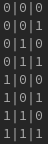
\includegraphics[scale=.8]{6.png}
\end{center}

\newpage

\section{Kesimpulan}
Setelah praktik mahasiswa dapat menjelaskan konsep array 3 dimensi, merencanakan struktur data dalam bentuk array 3 dimensi, mengaplikasikan array 3 dimensi.

\end{document}
